\chapter{Preparation}

The previous chapter introduced the concept of web applications and functional reactive programming (FRP). This chapter describes in detail the languages and libraries which will be used in the project. It shows the plans for the architecture of the applications to be produced, the infrastructure which will be used to support development and how testing will be carried out. It also contains a work plan for this implementation and testing.

\section{Requirements Analysis}
A successful implementation of this project should meet the following criteria:
\begin{itemize}
\item It should provide two or more significantly different web applications.
\item These applications must be cross-browser compatible.
\item Each must be compiled into JavaScript from a functional programming language and make use of reactive programming.
\item Use these applications to determine if these methods aid creation of web applications and what drawbacks they introduce.
\end{itemize}

\section{Starting Point}

I have had previous experience developing web applications in JavaScript. I found the language difficult to use, especially with respect to debugging. For example a common error would be that typing errors (such as misspelling variable names) would lead to uninitialised variables. This would still be valid JavaScript but the program would produce the wrong output. This section will outline the disadvantages of JavaScript and compare it to OCaml, a language which does not contain these drawbacks. 

\subsection{JavaScript}
JavaScript is used for client-side scripting in web pages. It is run on the local machine inside the browser environment and can access and modify the Document Object Model (\emph{DOM}), which is the browser's representation of the  objects on the current web page. By manipulating the DOM at run-time, JavaScript can be used to make interactive user interfaces and dynamic pages.

\subsection{OCaml}
OCaml is a language derived from Caml (Categorical Abstract Machine Language). Caml is a general purpose language which supports functional, imperative and object-oriented programming styles. It features a powerful type system that uses parametric polymorphism and type inference. This allows methods to be designed without having to explicitly declare the types of parameters or the result so functions can be reused with many different types of inputs. It also has pattern matching which can be used to direct control flow of the program through functions depending on their inputs~\cite{bib:caml}.

OCaml (Objective Caml) is a variant of the Caml language. It is an extension of Caml which adds an object-oriented layer and a module system. It is designed for use in developing commercial systems and is the most popular Caml derivative~\cite{bib:ocaml}.

\subsection{JavaScript vs OCaml}
In some ways JavaScript is very similar to OCaml. In both languages, functions are first class objects: they can be assigned to variables, passed as function parameters and invoked. However, the typing systems of OCaml and JavaScript are very different. OCaml types start off generic and become more specific each time they are used. In JavaScript variables themselves do not have a type and so can be reassigned to a value of any type. This can lead to programming errors because the user is not guaranteed to know the type of the object at any point. Indeed JavaScript uses type coercion which further complicates the situation. For example if a number is used in place of a boolean, zero will evaluate to \emph{false} and all other numbers to \emph{true}. Even worse, if a string is used as a boolean then the empty string represents \emph{false} and any non-empty strings (including the value "false''!) will evaluate to \emph{true}. Another difference is that OCaml is checked for errors at compile-time whereas JavaScript is checked at run-time. If a piece of code is not executed in a test-run, the user cannot be sure that it will succeed.

\section{Tools}
The previous section looked at and compared JavaScript and OCaml. This section will look at some libraries that can be used to write web applications in OCaml rather than JavaScript.

\subsection{ocamljs}
\emph{ocamljs}\footnote{\url{https://github.com/jaked/ocamljs}} is a modified version of the OCaml compiler written by Jake Donham\footnote{\url{http://jaked.org/}}. It uses the standard OCaml compiler up to the point when lambda code (see below) is generated; it replaces the last stage where byte code is generated and outputs JavaScript instead. Figure \ref{fig:ocamlc} shows the stages of the OCaml compiler and \emph{ocamljs}~\cite{bib:oreilly}.

\begin{figure}
  \center{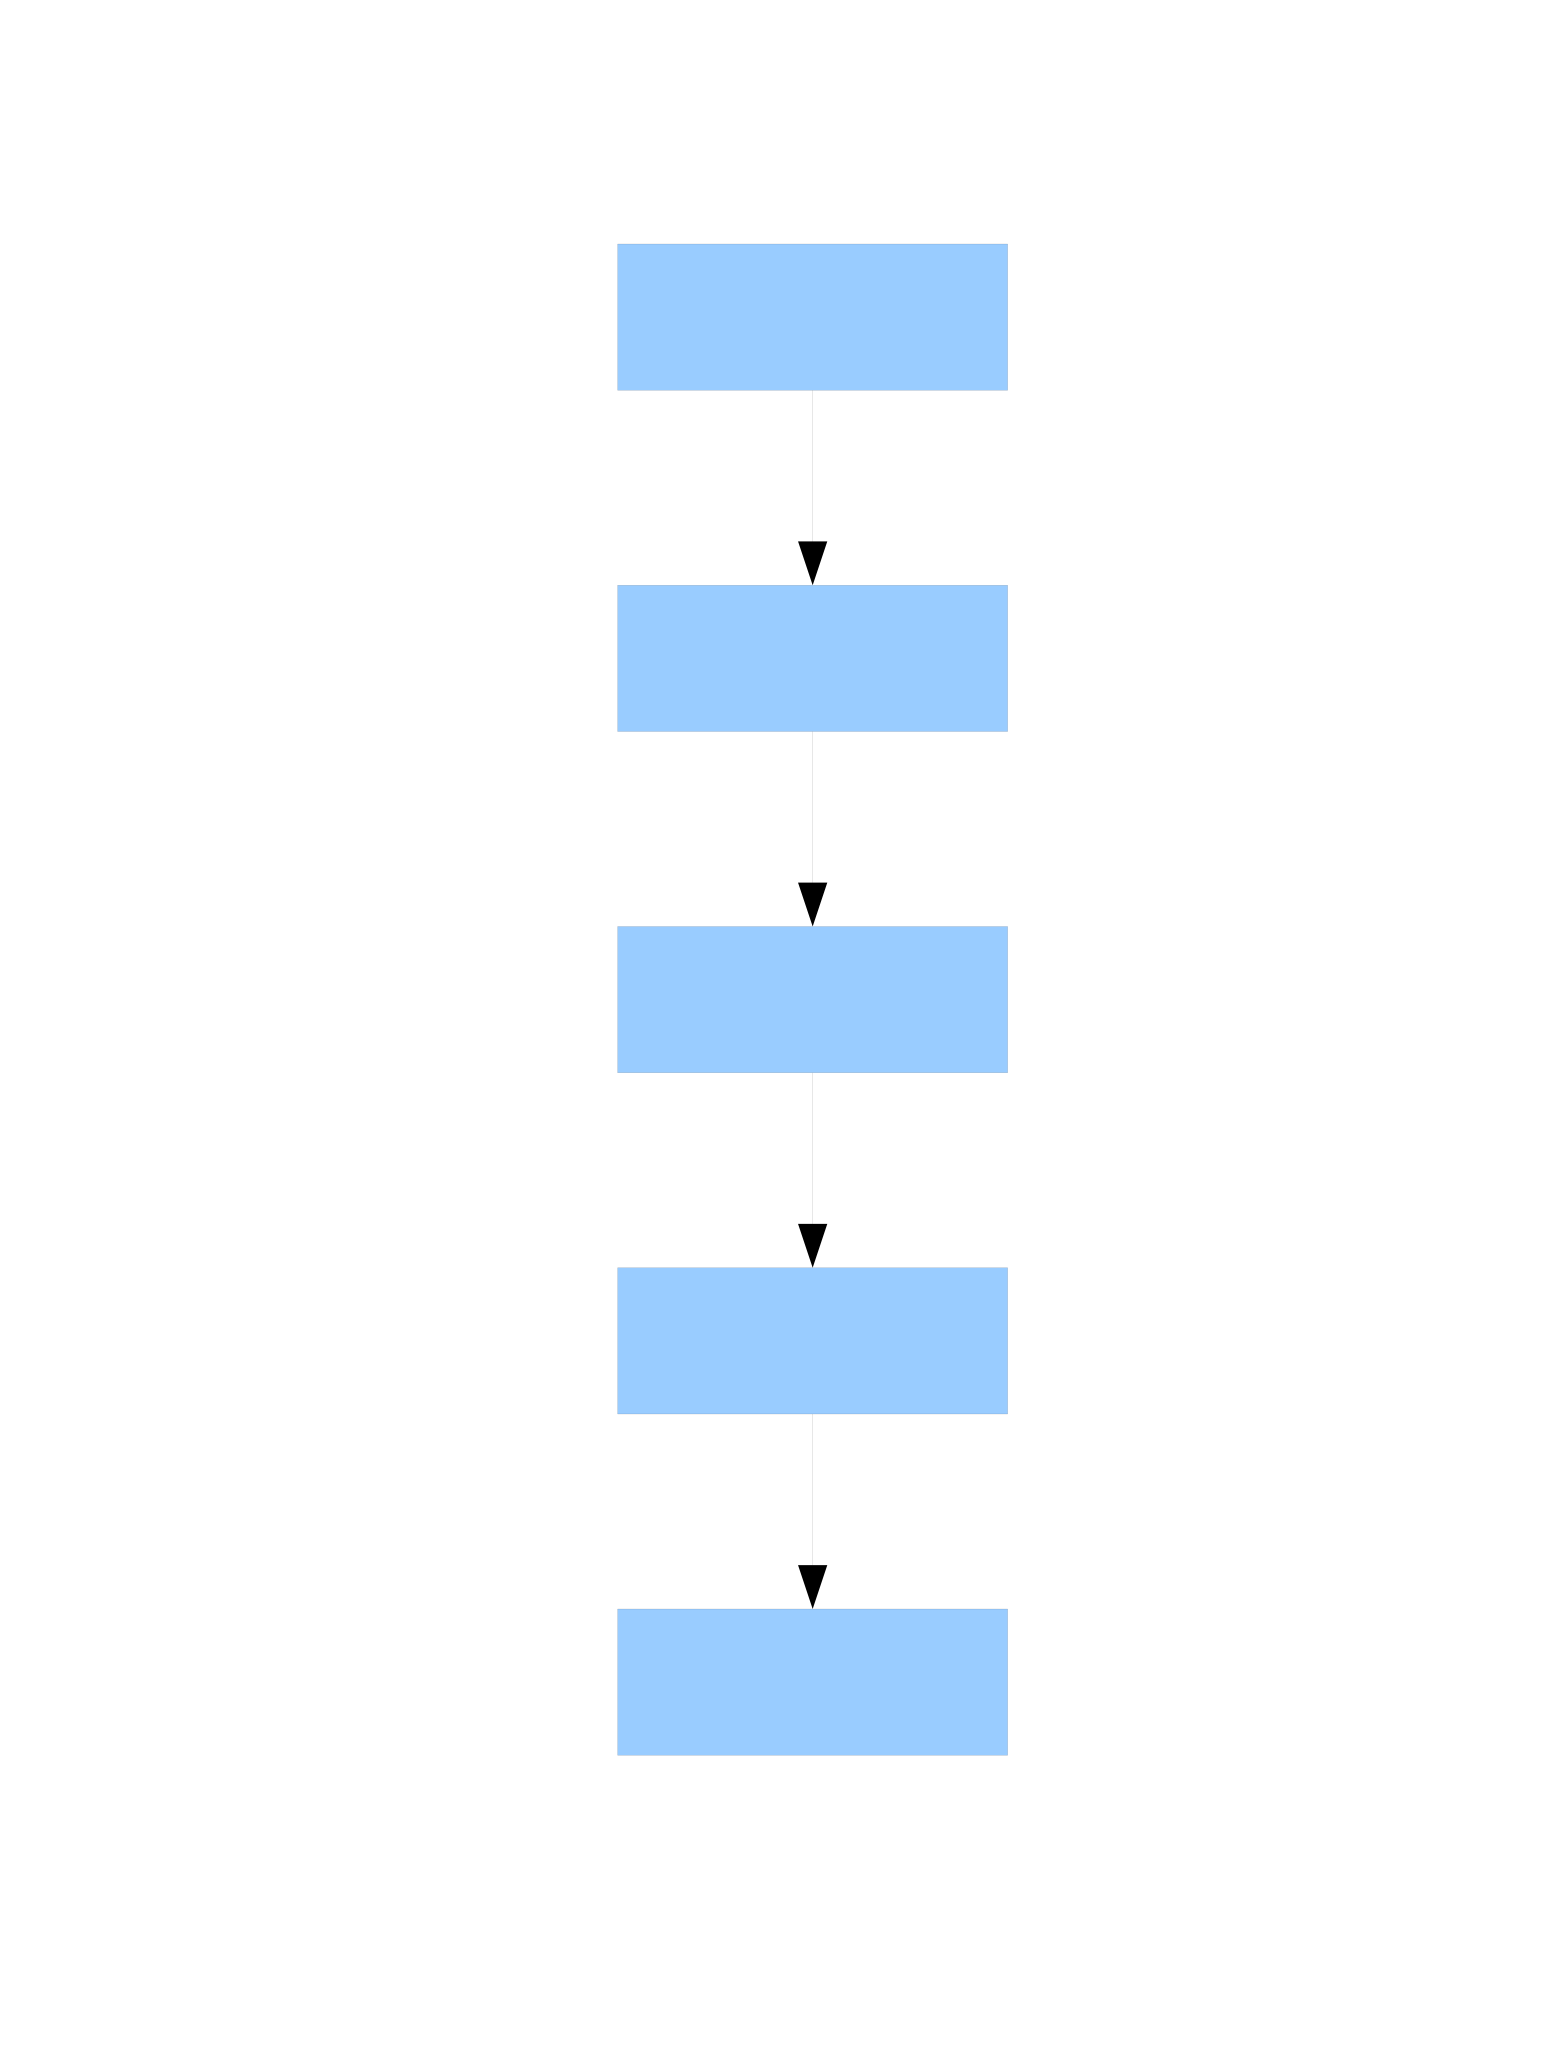
\includegraphics[scale=0.5]{images/ocamlc.pdf}}
  \caption{Stages of the OCaml compiler (ocamlc) and \emph{ocamljs}~\cite{bib:oreilly}}.
  \label{fig:ocamlc}
\end{figure}

\subsubsection{Lambda Code}
Lambda code is based on the $\lambda$-calculus, a notation invented by Alonso Church in the 1930s. It is used to describe the most basic ways that operators and functions can be combined. Conversion from mathematical functions to lambda-expressions is fairly straightforward~\cite{bib:lambda}. Here is a short example:

\begin{center}
$f(x) = x - 1$ becomes $\lambda x.x-1$
\end{center}

This may not look like a significant change but it makes the notation much closer to that used in programming. When there is more than one parameter for a function, multiple single parameter lambda-expressions are chained instead of having a multi-parameter lambda-expression. For example:

\begin{center}
$f(x,y) = x-y$ is $\lambda y.\lambda x.x - y$
\end{center}

Lambda code is very similar to $\lambda$-calculus. Consider the following OCaml program:

\begin{lstlisting}[caption={simple.ml},label=lst:simple-ml]
let f a b = a+b
let three = f 1 2;;
\end{lstlisting}

The OCaml compiler can output the lambda representation if the \emph{-dlambda} command-line switch is used. The lambda output for the above OCaml is shown below:

\begin{lstlisting}[caption={Lambda Code},label=lst:simple-lambda]
(setglobal Simple!
(let (
f/58 (function a/59 b/60 (+ a/59 b/60))
three/61 (apply f/58 1 2))
(makeblock 0 f/58 three/61)))
\end{lstlisting}

In this lambda code variables have been renamed. The lambda-expression part is \texttt{function a/59 b/60 (+ a/59 b/60)} which is equivalent to \texttt{$\lambda a.\lambda b.a+b$}.

\subsubsection{Lambda to JavaScript}
\label{lab:ocaml-js}
\emph{ocamljs} transforms lambda code into JavaScript. Functions and exceptions map simply into JavaScript. Integers and floats can be represented as a JavaScript \texttt{number} and booleans by the JavaScript \texttt{bool}. The standard library functions have been reimplemented in a static JavaScript file. Lists are implemented as a collection of nested JavaScript objects, each with two elements, \emph{0} is the value of the list at that position and \emph{1} is the tail of the list~\cite{bib:js_comp}.

Function applications are more complex. Functions in JavaScript require the correct number of arguments (and if less arguments are provided the rest default to null) whereas in OCaml, functions can receive more arguments (\emph{tail calls}) or less (\emph{partial application}). When we have a partial application, we want to return a closure and when we have a tail call, we want to apply the extra arguments to the result. This is solved using Simon Peyton Jones' \emph{eval-apply} method~\cite{bib:js_comp,bib:krivines_machine}.

\label{lab:eval-apply}
With the eval-apply scheme the caller is responsible for providing the correct number of arguments to a function. If there are not enough, a closure has to be created and if there are too many, the left over arguments are applied to the result of the function. This is implemented using the \texttt{apply} function outlined in Figure \ref{eval-apply}~\cite{bib:krivines_machine}.

\begin{figure}
  \begin{graybox}
  \begin{alltt}
f a\subs{1} ... a\subs{n} -> apply\subs{n}(f, a\subs{1}, ..., a\subs{n})

apply\subs{n} = \lam f x\subs{1} ... x\subs{n}
  match arity(f) with
    | 1   -> apply\subs{n-1} (f(x\subs{1}), x\subs{2}, ..., x\subs{n})
    | ...
    | n-1 -> apply\subs{1} (f(x\subs{1}, ..., x\subs{n}), x\subs{n})
    | n   -> f(x\subs{1}, ..., x\subs{n})
    | n+1 -> papp\subs{n+1,n}(f, x\subs{1}, ..., x\subs{n})
    | n+2 -> papp\subs{n+2,n}(f, x\subs{1}, ..., x\subs{n})
    | ...

papp\subs{p,q} = \lam f x\subs{1} ... x\subs{q}. (\lam x\subs{q+1} ... x\subs{p}. f(x\subs{1}, ..., x\subs{p}))
  \end{alltt}
  \end{graybox}
  \caption{Eval-apply implementation}
  \label{eval-apply}
\end{figure}

\subsubsection{ocamljs Example}
Below is the JavaScript code compiled from the OCaml example in listing \ref{lst:simple-ml}.

\begin{lstlisting}[caption={Compiled JavaScript},label=lst:simple-comp]
function () {
  var f$58 =
    _f(2, function (a$59, b$60) {
      return a$59 + b$60;
    });
  var three$61 = _(f$58, [ 1, 2 ]);
  return $(f$58, three$61);
}
\end{lstlisting}

\subsection{froc}

\emph{froc}\footnote{\url{https://github.com/jaked/froc}} is an OCaml library, also written by Jake Donham, for reactive programming in OCaml.

\subsubsection{Self Adjusting Computation}
\emph{froc} uses \emph{self adjusting computation} to push updates to input variables through data paths in the program. Self adjusting means that once the variable has been defined, the program will automatically forward changes to its dependencies. This is stored by the program as a \emph{dependency graph}.

\subsubsection{Dependency Graphs}
Given a set of variables and another set of dependencies (pairs of variables) a directed graph can be created where the variables form the nodes and the dependencies are the edges. This is a dependency graph and it is used by reactive programs to represent data-flow throughout the program.

\subsection{Behaviors and Events}
\label{lab:behavior}
Reactive programming uses two polymorphic data types, \emph{behaviors} and \emph{events}. \emph{behavior}s are values which vary over time. This could be a property such as the colour of an object or its width. Events are a series of time ordered values which correspond to real events such as mouse presses~\cite{bib:lambda}.

In order to use these time-varying variables \emph{froc} provides a way to create dependencies by \emph{binding} them to functions. Naturally this function is called \texttt{bind} and has the following interface:

\texttt{bind : 'a behavior -> ('a -> 'b behavior) -> 'b behavior}

This is a function which takes a \texttt{behavior} of type $\alpha$ and a callback function which converts an $\alpha$ to a $\beta$ \texttt{behavior} and returns a new \texttt{behavior}. Binding other \emph{behavior}s to a variable is how the dependency graph is constructed; whenever the dependent \emph{behavior}s change the callback function is invoked with the new values. There is also a syntax shortcut for bind, \texttt{\textgreater\textgreater=}.
\pagebreak
Any value can be converted into a \emph{behavior} using the \texttt{return} function:

\texttt{return : 'a -> 'a behavior}

Sometimes a callback which is a built in function might be required. Rather than wrapping it in a new function and calling \texttt{bind} there is another function called \texttt{lift} which does this automatically.

\texttt{lift : 'a behavior -> ('a -> 'b) -> 'b behavior}

There are also multiple argument versions of each function which allows variables to depend on more than one \emph{behavior} at once. Here are the two argument versions of \texttt{bind} and \texttt{lift}:

\texttt{bind2 : 'a behavior -> 'b behavior -> ('a -> 'b -> 'c behavior) -> 'c behavior}\\
\texttt{lift2 : 'a behavior -> 'b behavior -> ('a -> 'b -> 'c) -> 'c behavior}

Consider the following piece of OCaml:

\begin{lstlisting}[caption={Example with \emph{froc} \texttt{bind} (\texttt{\textgreater\textgreater=})}]
let x = return 1
let y = return 2
let z = return 3

let i0 =
    x >>= fun x ->
        y >>= fun y ->
            return (x + y)
let ans =
    i0 >>= fun i0 ->
        z >>= fun z ->
            return (i0 + z)
\end{lstlisting}

This program constructs a \emph{froc} \emph{behavior} which is the summation of three other \emph{behavior}s. Figure \ref{add_graph} shows the dependency graph that \emph{froc} holds internally for this program.

Figure \ref{if_graph} shows a more complex dependency graph. In this example if the value of \emph{behavior} \emph{b} was calculated before \emph{behavior} \emph{a} an exception could be raised. This example does not cause a divide by zero exception. The first thing this tells us about \emph{froc} is that it doesn't always execute every statement in the dependency tree, if an intermediate \emph{behavior} is unused \emph{froc} doesn't waste computation time on it. This is called \emph{lazy evaluation}. The second thing this tells us is that \emph{froc} evaluates \emph{behavior}s in a top-down order. It starts with the outputs and works out which \emph{behavior}s it needs to compute next from there~\cite{bib:froc}.

One final thing to mention is that \emph{froc} will not propagate changes to a \emph{behavior} if the callback returns the existing value of the \emph{behavior}. This is useful because it lets there be cycles in the dependency graph. If \emph{froc} did not have this property then a dependency graph with a cycle would not terminate.

\begin{figure}
  \centering
  \includegraphics[scale=0.5]{graphs/addition.png}
  \caption{Example dependency graph}
  \label{add_graph}
\end{figure}

\begin{figure}
  \centering
  \includegraphics[scale=0.5]{graphs/if.png}
  \caption{Example if-statement dependency graph}
  \label{if_graph}
\end{figure}

%\subsection{HTTP Server}
%An HTTP server is required to serve up a web page. At first a stock web server, such as \emph{Apache}, seemed like a good idea because it requires minimal setup. This is good for serving static content (such as HTML pages and JavaScript files) but dynamic content (such as time-dependent JSON messages) proves more tricky. In order to deliver interesting JSON data some server code is required. The two options are to use some sort of server side scripting which Apache can execute, although this requires learning a new language such as \emph{PHP} or to find an implementation of an HTTP server in a language this project is already using (such as OCaml) and modify it such that JSON data can be generated at run-time and delivered to the client.

%Using an OCaml HTTP server is the more sensible solution because it gives the greatest amount of time and lets me concentrate on writing the JSON generating code rather than getting stuck learning a new syntax. The OCaml web server I shall use is \emph{ocaml-cohttpserver}\footnote{https://github.com/avsm/ocaml-cohttpserver}.

\section{Architecture}

This section will describe the design of three web applications which will make up this project. Each application will use the common design architecture called \emph{client-server}. Client-server is normally based on many clients and one server. It is designed such that the amount of processing performed by the server after each request is minimal. The majority of the computation, which is usually involved in rendering the data as elements on a page, is performed by each client~\cite{bib:dist_arch}.

\begin{figure}
  \includegraphics[width=\linewidth]{images/client-server.png}
  \caption{Client/Server Architecture}
  \label{fig:client_server}
\end{figure}

\subsection{Log Viewer}
If we have a system where there are multiple threads which all run the same code, the log file will be interleaved with messages from each thread. This will make following the path of one thread through the logs difficult. An HTTP server is an example of a system with these properties. Each connection made to the server is run in a new thread and each of these runs almost the same sequence of code.

\textbf{Application 1}: Design a system using \emph{ocamljs} and \emph{froc} which could replace the logging module in a program to display the messages in a more helpful way.

\subsection{Dataset Graph}
Graphing is generally fairly straightforward. However, sometimes we wish to represent data which has more than two variables. This is difficult on a graph with just two axes. One way we can represent a third axis is by mapping it to time. The graph can show the values for the other two variables with the third one fixed. A \emph{play} feature can be used to show all of these graphs with the third variable changing over time.

\textbf{Application 2}: This application will show data with three variables, one on each axis and one which is varied using a \emph{play} function. 

\subsection{Heat Map}
A heat map is another type of graph. Instead of varying in the X and Y axis, points remain fixed. Each point varies over time in colour or \emph{heat}. As the time changes each of the data points updates its colour to the new value.

\textbf{Application 3}: Create an application which displays data about energy usage over time for a number of rooms in a building.

\section{Infrastructure}

This section describes the tools that will be used to help with development, version control, source code back-up and compilation of the project.

\subsection{Version Control}
Version control is very important for a software project. It involves breaking the project into a number of changesets. Each change consists of differences to files along with a brief description explaining what changes were made. The idea is that the code is in a consistent state before and after each commit. This is often used in conjunction with pushing changesets to a remote server which is regularly backed up. As a consequence if files become corrupted, deleted or changed in such a way that work has been undone the files can be reverted to a working copy\footnote{It turned out to be very useful I had used version control on this project because a failed operating system upgrade left my machine unbootable. Once I had it working again I only needed to clone the repository again and I could continue working where I left off.}.

There are many version control systems. \emph{Git}\footnote{\url{http://git-scm.com/}} is the one used for the \emph{ocamljs} and \emph{froc} projects. It has the required functionality and there is a free to use service run by \emph{GitHub}\footnote{http://www.github.com} on condition that your code is publicly viewable and anyone can fork your repository. The \emph{GitHub} service also provides some social networking features which allow other developers to follow changes to repositories they are interested in. The repository for this project can be found at \emph{https://github.com/hhughes/ocaml-frui}.

\subsection{Compiling the Project}
The \emph{GNU Make}\footnote{\url{http://www.gnu.org/software/make/}} system will be used to perform compilation of the project. Make uses shell scripts and dependencies to compile just those parts of the project which have changed since it was last compiled. Compilation of this project is likely to be reasonably quick but it is good practice to use Make for when projects become larger. Make is also a commonly used and simple tool. It is likely that those who clone this repository will already be familiar with the tool.

\section{Development Model}
This project will use the \emph{waterfall model} of development. This method separates out each stage of development which simplifies the design-implement-testing process~\cite{bib:royce}. The maintenance stage has been removed from the original model because that is beyond the scope of this project. Figure \ref{fig:waterfall} shows the stages of the waterfall model as used in this project.

\begin{figure}
  \centering
  \includegraphics[scale=0.5]{images/waterfall.pdf}
  \caption{Waterfall development model (with \emph{maintenance} stage removed}
  \label{fig:waterfall}
\end{figure}

\section{Testing}
In order to test the applications written using \emph{ocamljs} and \emph{froc}, each application has to be recreated using handwritten JavaScript. These implementations should provide the same functionality and use as close to the same algorithms as possible. Each version of each application will be tested using dummy input data and the average execution time of the JavaScript in each case will be used as a comparison. Each application should also be tested on at least two web browsers which use different JavaScript engines (for example \emph{Google Chrome}\footnote{\url{http://www.google.com/chrome/}} uses \emph{V8}\footnote{\url{http://code.google.com/p/v8/}} and \emph{Mozilla Firefox}\footnote{\url{http://www.mozilla.org/firefox}} uses \emph{SpiderMonkey}\footnote{\url{https://developer.mozilla.org/en/SpiderMonkey}}). This is because different browsers will optimise different parts of the code. A note should also be made of the estimated number of man-hours invested in both the \emph{ocamljs} and pure JavaScript implementations to compare the \emph{ease} of writing the code.

Micro-tests (e.g. implementations of simple algorithms such as \emph{quick-sort} or \emph{matrix multiplication}) may also be required if test results from the web applications are not significant.
\vfill

\section{Gantt Chart}
\begin{center}
\includegraphics[angle=270]{charts/gantt.pdf}
\end{center}
